\section{Anonymized Dataset Producing Libraries}

As mentioned earlier, an other possible output of a mechanism that adds D.P. to a dataset can be the dataset itself, after being anonymized using certain algorithms that meet the criteria of D.P.

This technique does not yet have many different implementations, mostly due to the success of the previous model shown, as well as the difficulty, the computer power needed and the poor quality of the result being produced.

Producing an anonymized dataset is the way to go if someone is using earlier forms of data privacy, such as \textbf{k-anonymity}, \textbf{l-diversity} etc, which we are going to analyze moving forward. However, in order to cover the needs of D.P., several adjustments have to be made. The main idea behind all those libraries, lay behind a theorem, presented in [4], that mixes the use of those previously mentioned techniques with D.P.

In this Thesis, we are going to examine the \textbf{ARX tool}, a tool for data anonymization, that supports the method that we are trying to implement. We are going to analyze this tool, and perform similar testings as in IBM. 

ARX is a tool for data anonymization, that in general, takes a dataset as an input, applies  privacy models, and produces an anonymized version of this dataset, thus offering protection to its members. The Menu of the ARX tool can be seen in the following \textbf{Figure 3.7.}

\begin{figure}[!htb]\centering
    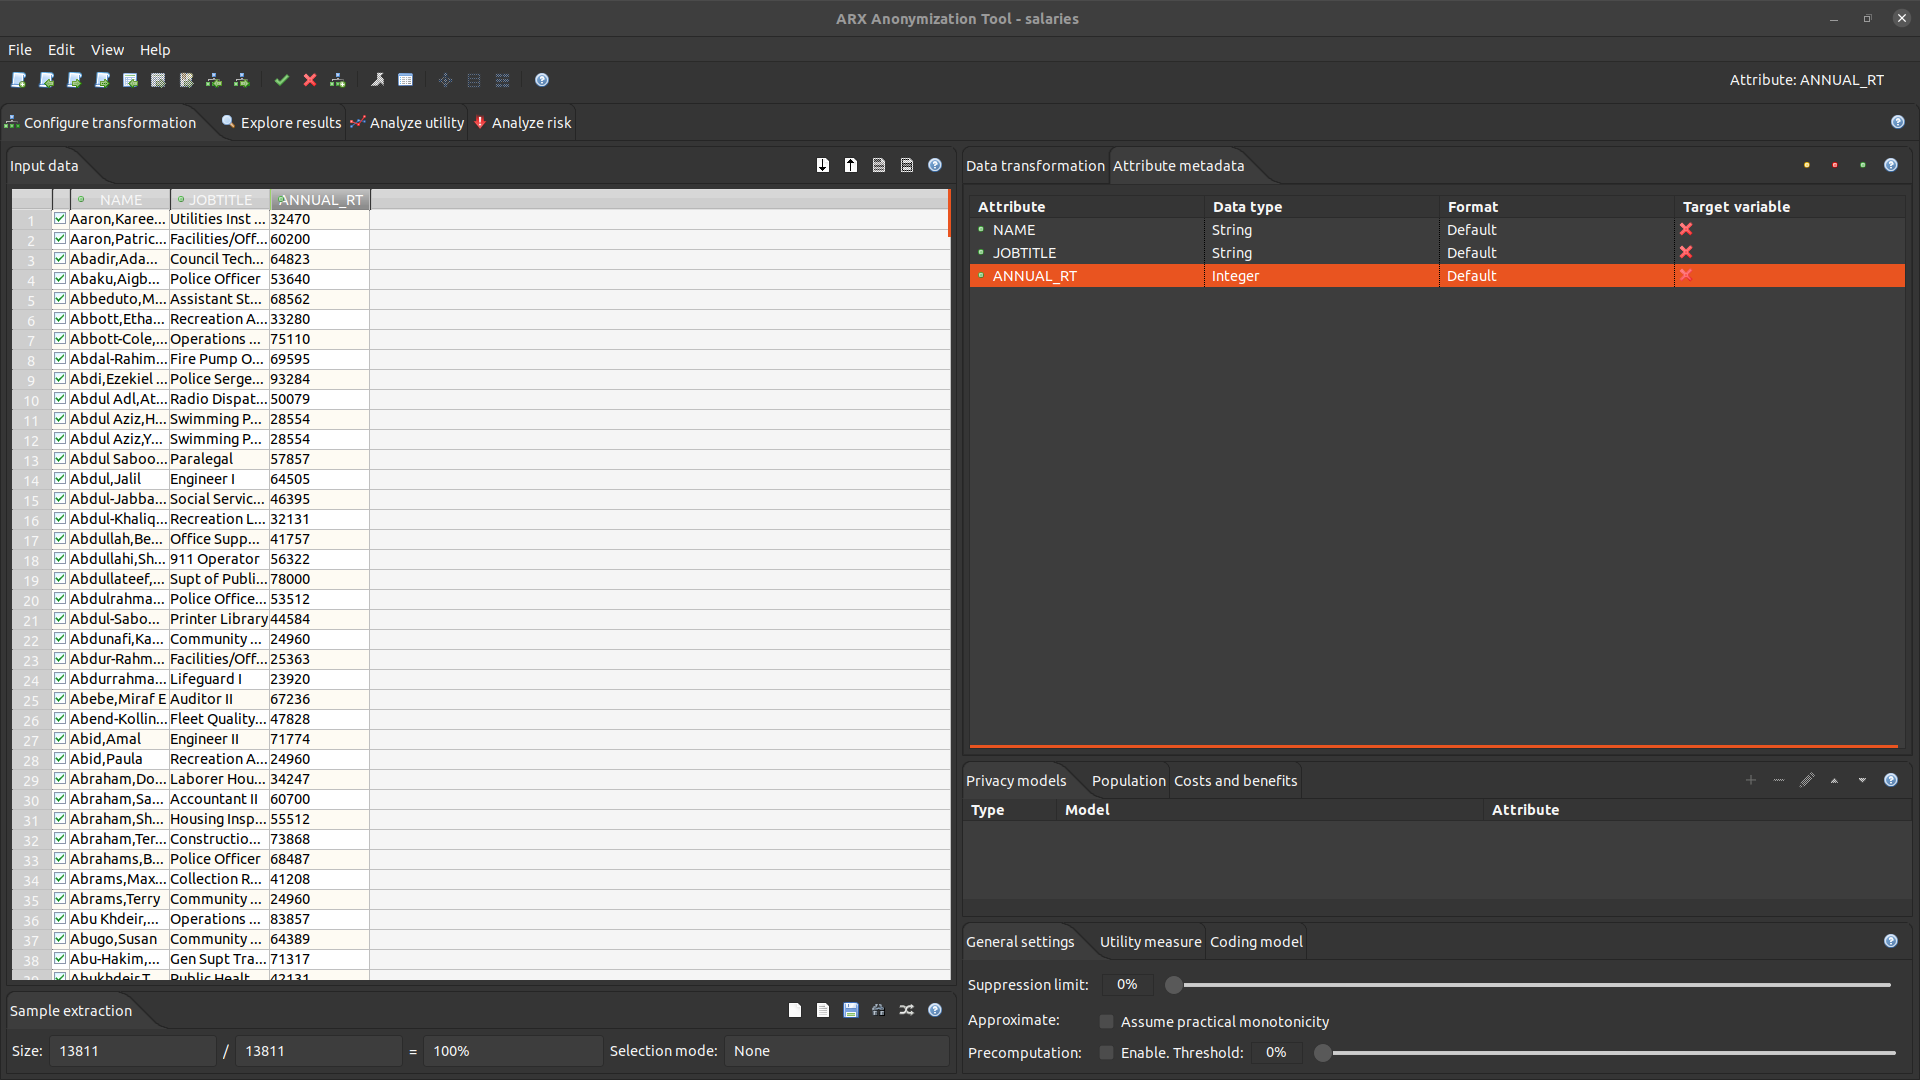
\includegraphics[width=0.9\textwidth]{images/arx_tool.png}
    \caption{The ARX GUI tool}
\end{figure}

At its core, ARX uses a highly efficient globally-optimal search algorithm for transforming data with full-domain generalization and record suppression. The transformation of attribute values is implemented through domain generalization hierarchies, which represent valid transformations that can be applied to individual-level values.

\subsection{Classic Privacy Models}

The ARX tool offers standard privacy models that are tested in theory and are widely used to ensure anonymity given a plain dataset. Those consist of the implementation of the following protocols:

\begin{itemize}
    \item \textbf{K-anonymity}: A well-known privacy model that aims to protect datasets from re-identification in the prosecutor model. A dataset is $k$-anonymous if\textbf{ each record cannot be distinguished from at least $k-1$ other records regarding the quasi-identifiers.} Each group of indistinguishable records forms a so-called equivalence class. 
    \item \textbf{l-diversity}: This privacy model can be used to protect data against attribute disclosure by ensuring that each sensitive attribute \textbf{has at least $l$ "well represented" values in each equivalence class}. Different variants, which implement different measures of diversity, have been proposed.
\end{itemize}

Moreover, the tool uses some simple concepts of processing a dataset:

\begin{itemize}
    \item \textbf{Random Sampling}: A method of sampling that utilizes some form of random selection. In order to have a random selection method, we must set up some process or procedure that assures that the different units in the population have equal probabilities of being chosen.
    \item \textbf{Attribute Generalization}: Generalizing a column of the dataset, based on its values. The applications of attribute generalization depend on the type of records (eg. integers, ranges etc).
    \item \textbf{Record Suppression}: Deletion of a specific row on the input dataset.
\end{itemize}

Those are some techniques that are not going to be analyzed and tested in this thesis, however, if combined with D.P. can produce interesting results. Specifically, according to [4], the following theorem applies:

\textbf{Random sampling} with probability $\beta$ followed by \textbf{attribute generalization} and the \textbf{suppression} of
every record which appears less than k times \textbf{satisfies $(\epsilon, \delta)$ differential privacy} for every $\epsilon \geq -ln(1-\beta)$ with 
$$\delta = \max_{n:n \geq n_m} \sum_{j>\gamma_n}^{n}f(j;n,\beta)$$

where $n_m = \frac{k}{\gamma} - 1$, $\gamma = \frac{e^\epsilon-1+\beta}{e^\epsilon}$ and $f(j;n,\beta) = {n \choose  j} \beta^j(1-\beta)^{n-j}$.

In order to achieve attribute generalization, ARX uses the so called \textbf{hierarchies}. They are either imported from a csv file, or being hard-coded into the API, and they are used in order to generalize a sensitive field. An example is given in \textbf{Table 3.4}. The subject to generalize is the age of a person. Let's see the values as they proceed through generalization.

\begin{table}[!htb]
    \centering

    \caption{Generalization of data using hierarchies}
    \label{numbers}

    \begin{tabular}{| c | c | c | c |}
      \hline 
      $1^{st}$ level & $2^{nd}$ level & $3^{rd}$ level & $4^{th}$ level\\
      \hline
      1 & 0-4 & 0-9 & *\\
      \hline
      3 & 0-4 & 0-9 & *\\
      \hline
      5 & 5-9 & 0-9 & * \\
      \hline
      10 & 10-14 & 10-19 & *\\
      \hline
      18 & 15-20 & 10-19 & *\\
      \hline
    
    \end{tabular}
\end{table}

\subsection{Conducting D.P. Testings}

ARX provides a cross-platform graphical tool, that supports many different ways of anonymizing data, as well as an API that delivers those data anonymization capabilities to Java programs. We are going to use the latter, in order to create our own scripts for testing the tool and its accuracy.

In order to test the accuracy of the models used by ARX, we are going to run simple queries, on the datasets produced by the anonymization process. We want to eliminate the probability of extremely high noise generation, thus we are going to run the anonymization tool multiple times, and the output dataset will be constructed by the mean values of the fields.

As show on the above matrix, ARX hierarchies tend to treat every type of value as a string, in order to replace it with an interval. This is not  desirable when applying the testings we mentioned. Thus, we had to come up with a better solution of defining hierarchies. The ARX GUI provides a wizard that gives a variety of choices so the user can easily create a hierarchy for many data types.

Another challenge is the number of layers that we are going to use, meaning how far our anonymization will proceed. In each layer, the number of same records increase exponentially, thus we do not want to apply many layers, in order for our results to be accurate, and the output dataset to be readable.

Given the help from Dr. Fabian Prasser, one of ARX's creators, we opted to treat the integer values as numbers, and in each level:
\begin{itemize}
    \item Group the rows by 2
    \item Apply a function according to the query we want to ask.
\end{itemize}
 
For example, if we want a counting query, the best option would be to apply an \textbf{arithmetic mean} function to the group, thus the sum, the mean, the variance etc will be the same. The way that ARX preserves D.P. with those settings, is by record suppression. If that was not the case, the results would be identical to the input dataset. However, now, the output dataset will differ because of its lack of some rows of the input.
 
Regarding the layers problem, we opted to use 4 layers of anonymization, the last of whom will be the * value, meaning that every record is inseparable. We do not want this to happen early in our anonymization, but we do not want it to never happen either, because then we would have a privacy leak, if the dataset was too small.

The creation of the hierarchies for the salary column, can be shown in \textbf{Figure 3.8}, taken from the ARX GUI Hierarchy Creation Wizard.

\begin{figure}[!htb]\centering
    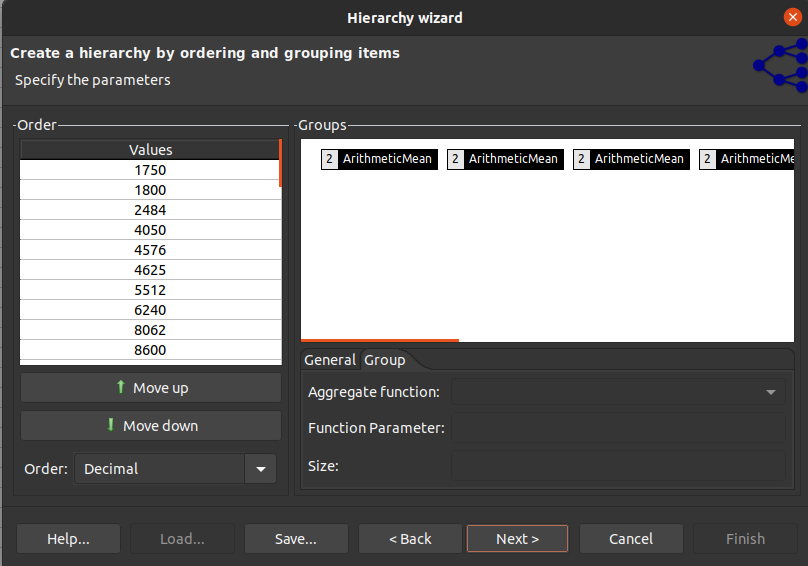
\includegraphics[width=0.8\textwidth]{images/hierarchies.png}
    \caption{Creating an Hierarchy using ARX GUI}
\end{figure}


\subsection{Metrics Used}
We are going to test the applicability of the already given ARX mechanisms on a numerical dataset. Our goal is to run basic queries, such as mean value on the dataset's records. We are going to do that first by applying no DP at all, and then by using the API that is presented by ARX, helped by a simple java script that was built for this purpose.


\subsection{The identity of the testing Dataset}
The dataset that we are going to be looking at, contains sensitive data regarding NBA players' \textbf{salaries} from the year 1990 until today. It also states other info about them, such as their \textbf{age}, their\textbf{ current team }and their \textbf{position}. This particular data is not considered sensitive, as those numbers are widely available, however, when it comes down to certain people's salaries, applying D.P. in order to preserve their privacy is crucial.

\subsection{Process of running the queries}
As we have earlier noted, the application of D.P. in ARX is rather complicated, let along the use that we are interested in: We want the output dataset to have numerical values in the earnings' column, in order to apply queries. 

For each column of the dataset, we have defined our own hierarchies. For every column except the `Salaries` one, this hierarchy is semantic, like the ones presented in our intro.

For the salaries column, with it being our goal to analyze, we opt to use the construction mentioned in our solution in the intro. We created 7 layers, in order to give the algorithm the ability to anonymize the dataset without the values being converted to `*`.

A sample of the result of the creation of the Salaries hierarchy is presented in \textbf{Table 3.5}, while the whole file is available in the GitHub distribution of the results of this Thesis.

\begin{table}[!htb]
    \centering

    \caption{Hierarchy Levels created}
    \label{numbers}

    \begin{tabular}{| c | c | c | c | c|}
      \hline 
      $1^{st}$ level & $2^{nd}$ level & $3^{rd}$ level & ... & $7^{th}$ level \\
      \hline
        79.568  &	291.029 & 500.776 &   	... &	*\\
              \hline
        502.491 &	291.029 &	500.776 &... &	*\\
              \hline
        522.738 &	710.524 &	500.776 &...	&   *\\
              \hline
        898.310 &	710.524 &	500.776 &... &	*\\
              \hline
        1.000.000 &	1.114.013 &   1.220.739 &...&	*\\
              \hline
        1.228.026 &	1.114.013 &   1.220.739 &... &	*\\
              \hline
    \end{tabular}
\end{table}

Next up, we are going to setup the use the ARX API, which requires us to specify some variables in order to run Differential Privacy. Those variables are defined in the above Java code, and are those that were use in the actual testings.

\bigskip
\bigskip
\bigskip
\bigskip
\begin{lstlisting}[
basicstyle= \footnotesize,
language=Java]
    EDDifferentialPrivacy criterion = new EDDifferentialPrivacy(2d, 1d / Rows);

    ARXConfiguration config = ARXConfiguration.create();
    config.addPrivacyModel(criterion);
    config.setSuppressionLimit(1d);
    config.setHeuristicSearchStepLimit(100);
    ARXResult result = anonymizer.anonymize(data, config);
\end{lstlisting}
\bigskip


The basic principles that were followed for the above definitions are based on the following instructions and guidance by the ARX Tool documentations:
\begin{itemize}
    \item The delta value should not be 0, but is suggested to be set lower or equal than the reciprocal of the number of records.
    \item A suppression limit should be set, preferably to 1.
    \item In order to improve the quality of the data produced, a heuristic search step limit should be set, in order to tweak the ARX search algorithm that handles data suppression.
\end{itemize}

Additionally, following the same principles as with the IBM library, we are going to run the D.P. query multiple times before reporting its value. We are going to do so, because the amount of noise generated can be extreme, and because of the low bounds of the heuristic search that we have set. We chose to run each query 1000 times, and then report the mean value of those runs as the result produced by the mechanism.

Because of the structure of the result of the ARX mechanism (a dataset containing numerical values), we can only run queries like \textbf{sum} and \textbf{mean}. There is no point in running a min or max query: we already know that the result will not be accurate. Thus, we are going to try to run a\textbf{ mean value} numerical query in the anonymized dataset. The function we are using in order to run this typed of queries is the following:
\bigskip
\clearpage
\begin{lstlisting}[
basicstyle= \footnotesize,
language=Java]
protected static double run_query(ARXResult data, int targetColumn) {
	// iterator that we are going to use to access the data
	final Iterator<String[]> itHandle = data.getOutput().iterator();
	
	// result of the query
	double result = 0d;
	// length of the dataset
	int totalRecords = 0;
	
	// ignore the name of the column
	String[] name = itHandle.next();
	if (name.length <= targetColumn) {
		System.out.println("Target column out of bounds\n");
		return 0d;
	}

	// iterate through all the values in the dataset
	while(itHandle.hasNext()) {
		String[] next = itHandle.next();
		// check that our target position is legal
		String string = next[targetColumn];
		if (!string.equals("*")) {
			result += Integer.parseInt(string);		
			totalRecords++;				
		}
	}
    // return the __mean__ of the dataset
    return result / totalRecords;
}
	
\end{lstlisting}
\bigskip

Finally, before running the queries, we must mention that the dataset size should be significant, as our own contains thousands of columns. The dataset size is a critical parameter when applying D.P., while being even more essential during the use of the ARX tool.

\subsection{Statistical Queries}

As shown by the above Java function, our testings can support every type of statistical queries, such as \textbf{mean value}, \textbf{sum}, and \textbf{average}. However, due to the computer power required and the similarity of the results that those queries produce, we will focus our testings solely to the mean value query.

Given the dataset previously analyzed, the true mean value of the salaries column of the dataset is $\$2.868.981,32$. This will be the value that we are going to use in order to examine the accuracy of the D.P. results.

\subsubsection{Running with fixed parameters}

We are going to conduct our first test by anonymizing our dataset using the default parameters, as we set ε $ = 1$ and δ $ = \frac{1}{12377}$.  The results are shown in the following table.


\begin{table}[!htb]
    \centering

    \caption{Mean value query in ARX with default parameters}
    \label{numbers}

    \begin{tabular}{| c | c |}
      \hline 
        Non-DP result & DP Result \\
      \hline
        $\$2.868.981,32$ & $\$2.860.215,6$\\
      \hline
    \end{tabular}
\end{table}

We observe that the query results, are somewhat close: We are in the range of millions of dollars, and the ARX mechanism only fails to approach the result by 8 thousand. This is not of course close to what the IBM library computed, but it is still a reliable result, given all the downsides of this type of anonymization.


\subsubsection{Running with different epsilon values}

Next up, in order to determine if ARX follows the rules of D.P., we should try anonymizing the dataset for different values of epsilon, just like we did with the IBM library.

We observed during our initial runs that if the epsilon value rises above 2, the algorithm faces certain problems, that will be analyzed moving forward. With that being the case, the epsilon values chosen to conduct the measurements are in the range $[0.2, 1.6]$. The results from our testings are shown in the above \textbf{Figure 3.8.}

\begin{figure}[!htb]\centering
    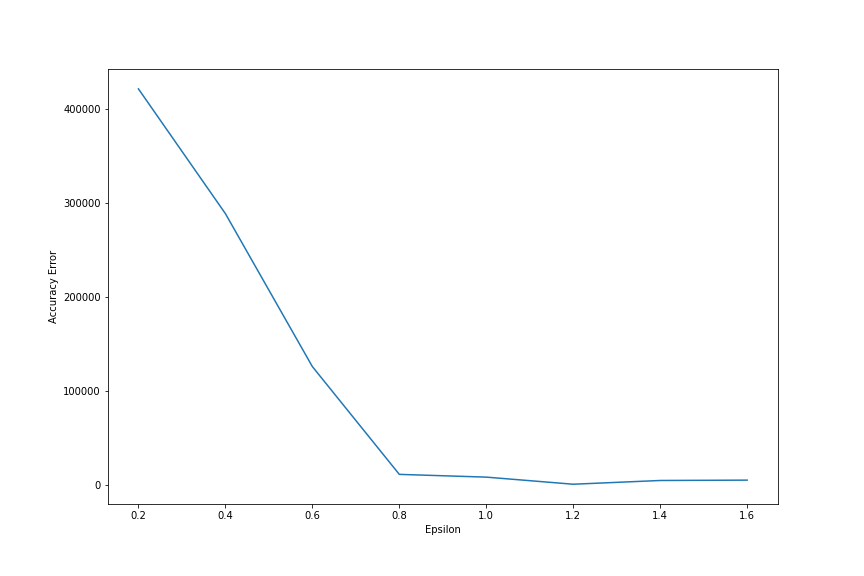
\includegraphics[width=1\textwidth]{images/arx_accuracy.png}
    \caption{Accuracy Error results for increasing values of epsilon}
\end{figure}

As we can see, the plot does not behave as expected, but it is in the right direction. We are used to seeing a more logarithmic-like plot, but here we observe that when the epsilon rises above `0.8`, the results are similar. We can not compare the results with the Laplace noise distribution, because of the way that the results are produced. 

We generate the answers given by asking the query in the output dataset. Without its records being suppressed, the result dataset would have been perfect, because of the transformation of the data. However, when suppressing many records (nearly 10\% each time), the result could be severely altered, and thus the error plot, as we saw, is quite unpredictable.


\subsection{Observations regarding the Algorithm}

During our testings in the dataset using the ARX mechanism, we observe the following regarding its behavior in the DP queries:

\begin{itemize}
    \item The epsilon variable if raised above 2,5, makes the algorithm \textbf{extremely slow}, to the point that it does not respond after minutes of execution. This makes sense, if we take into consideration that when epsilon increases, the accuracy gets better. Thus, the algorithm performs extreme searching techniques in order to find which records to suppress, resulting into slow execution.
    \item In order for the algorithm not to produce only *(the last level in our hierarchies) in our target column, we set each of the other columns as \textbf{non sensitive} in their definition.
    \item As the epsilon values rise, \textbf{the accuracy gets better}, as it is supposed to be, according to the DP principles.
    \item While the dataset has multiple columns, the algorithm usually fails to present all of them with anonymized values, and just reports * in each row. This could have been a result of the high \textbf{Heuristic Search Step Limit}, which was by default set to maximum. Despite us lowering its value, the phenomenon persists.
\end{itemize}

\subsection{Conclusion}

While researching the ARX mechanism we came to the conclusion that it is for sure a whole different approach in Differential Privacy compared to the other libraries that we studied. With that being the case, it has some advantages and some disadvantages. Its main advantages are the following:

\begin{itemize}
    \item The result of the mechanism is a \textbf{handy dataset} that the user can handle in multiple ways and gain more information than just the result of a query.
    \item The result \textbf{can be iterated}, thus giving the option to the user to run the query in a smaller subset of the rows, while it being differential private.

\end{itemize}

On the other hand, the main disadvantages are:
\begin{itemize}
    \item The result can be misleading, because of the \textbf{big accuracy error produced}.
    \item The algorithm \textbf{requires a rather big dataset} in order to run properly, while other libraries perform just fine with smaller datasets.
    \item The algorithm is difficult to implement, as you have to create a self-made function for every query, and moreover tune many parameters if you want to run differential privacy.

\end{itemize}
